This chapter formalises the conceptual choices behind Tino V2: a ROS2-centred architecture using RTABMap for mapping, Oak‑D Pro for stereo depth, UWB for absolute positioning, and a YOLOv11+TensorRT pipeline for real-time human pose estimation. The chosen sensor selection approach balances metric accuracy, runtime performance and practical robustness demonstrated during the development phase.

\section{System Requirements Analysis}
Understanding the limitations and capabilities of the original Tino robot system provides essential context for the design requirements that guided Tino V2 development. This analysis examines the legacy system architecture and identifies specific enhancement requirements that shaped the technological choices presented in subsequent sections.

\subsection{Legacy System Architecture}
The original Tino robot, developed as part of previous research in social robotics~\cite{cardillo2024thesis}, utilized a Raspberry Pi-based control architecture with inherent computational limitations. The system employed a Triskar omnidirectional base providing three-degree-of-freedom mobility through three independently controlled wheels arranged in a triangular configuration.

While this omnidirectional configuration offered excellent theoretical maneuverability for social interaction scenarios, practical deployment revealed significant reliability issues under the robot's operational weight. Wheel degradation and mechanical wear patterns limited system reliability and required frequent maintenance interventions.

The legacy sensor suite was extremely limited, consisting only of a basic Pi camera used exclusively for video streaming to remote operators. The system lacked any environmental sensors or perception capabilities, with the camera providing raw video feed without any on-board processing for computer vision, object detection, or environmental analysis.

\subsection{Software Architecture Limitations}
The original software architecture employed monolithic Python scripts with limited modularity and debugging capabilities. This approach made system maintenance and feature development challenging, particularly when attempting to integrate new sensing modalities or advanced control paradigms.

Communication between system components was handled through simple serial interfaces without the robust messaging frameworks required for complex multi-sensor systems. The absence of standardized robotics frameworks made it difficult to leverage existing libraries and tools for advanced robotics capabilities.

\subsection{VR Integration Requirements}
The motivation for Tino V2 development arose primarily from requirements for VR integration that were not feasible within the original system constraints. VR teleoperation demands real-time processing of commands, sophisticated sensor fusion for accurate localization, and low-latency communication protocols.

The legacy system lacked the computational capabilities required for real-time computer vision processing, advanced SLAM algorithms, or sophisticated human detection and pose estimation systems. These limitations prevented implementation of the data processing pipelines necessary for meaningful VR integration.

Most critically, the original architecture could not support the real-time sensor fusion and environmental mapping capabilities required to provide accurate robot localization and human pose data to VR systems. Without these capabilities, meaningful VR-mediated social interaction remained impossible.

\subsection{Identified Enhancement Requirements}
Analysis of the legacy system revealed several critical enhancement requirements that motivated the comprehensive redesign undertaken in Tino V2:

\begin{itemize}
\item \textbf{Computational Platform Upgrade}: Migration from Raspberry Pi to more powerful embedded computing platforms capable of real-time AI processing and sophisticated sensor fusion.

\item \textbf{Advanced Localization Systems}: Implementation of robust SLAM capabilities with map persistence and reliable relocalization for consistent spatial awareness.

\item \textbf{Human Detection and Pose Estimation}: Integration of real-time computer vision systems capable of detecting and tracking human pose for VR representation.

\item \textbf{Modular Software Architecture}: Development of ROS-based modular architecture enabling easier integration of new capabilities and robust debugging.

\item \textbf{VR Communication Infrastructure}: Implementation of low-latency communication systems capable of real-time data exchange with VR environments.

\item \textbf{Mechanical Reliability Improvements}: Redesign of the mobility platform to address reliability issues while maintaining expressive movement capabilities.
\end{itemize}

These requirements collectively defined the scope and objectives for the Tino V2 development project, establishing the foundation for the technological solutions presented in the following sections.

\section{Technology selection rationale}

The selection of the Tino V2 technology stack followed a requirements-driven process that balanced perception accuracy, real-time constraints on embedded hardware, integration complexity with legacy code, and operational robustness for prolonged experiments. The priorities used to evaluate candidate technologies were:

\begin{itemize}
	\item \textbf{Functional accuracy}: localization and human pose estimation must be precise enough to feed the VR system with metric robot pose and 3D human joint positions.
	\item \textbf{Real-time performance}: the chosen algorithms must run on the onboard compute (NVIDIA Orin Nano) with low latency to satisfy VR and teleoperation requirements (target end-to-end perception latency $<$ 100 ms where possible).
	\item \textbf{Integration and maintainability}: preference for solutions with ROS2 support, stable persistence (map save/load and relocalization), and reasonable build effort on ARM64.
	\item \textbf{Robustness and recoverability}: the system must tolerate temporary sensor dropouts, relocalize from different viewpoints, and provide fallbacks to reduce mission-critical failures.
\end{itemize}

Using these criteria, the final choices were: RTABMap for SLAM and map management, an Oak-D Pro (DepthAI) stereo camera for visual + depth input, UWB anchors for absolute positioning, and a YOLOv11-based pose estimation pipeline accelerated with TensorRT for real-time skeleton extraction. The integration of these technologies within the overall system architecture is shown in Figure~\ref{fig-system-architecture}, with the justifications for each component summarised below.

\begin{figure}[H]
	\centering
	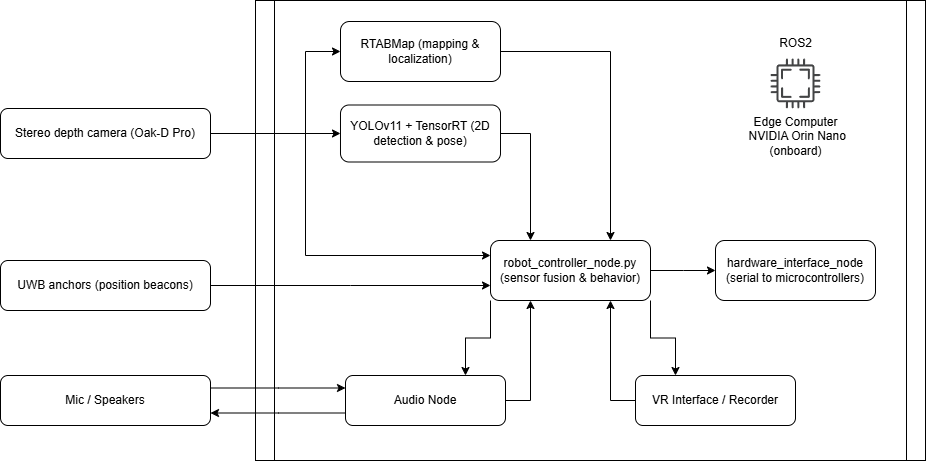
\includegraphics[width=0.85\linewidth]{Images/system_architecture.png}
	\caption{High-level system architecture for Tino V2.}\label{fig-system-architecture}
\end{figure}

\subsection*{Why RTABMap over ORB‑SLAM3 and SVO}
RTABMap provides robust multi-session map persistence, reliable relocalization and first-class ROS/ROS2 integration. During early experiments ORB‑SLAM3 and SVO presented compilation fragility on ARM64 and unstable atlas save/load behavior with the available cameras. RTABMap demonstrated stable map saving/loading and dependable relocalization in practice, making it preferable for a system where map reuse and long-term experiments are required.

\subsection*{Why Stereo Cameras and Oak‑D Pro}
Stereo cameras were selected over both monocular cameras and structured light depth sensors as the primary depth sensing technology due to their fundamental advantages for mobile social robotics applications. Compared to monocular cameras, stereo vision provides direct metric depth estimation without requiring additional sensors or complex monocular depth estimation algorithms that often lack the accuracy needed for precise 3D human pose reconstruction. While monocular depth estimation using neural networks has advanced significantly, it still suffers from scale ambiguity and reduced accuracy at varying distances, making it unsuitable for the metric precision required by VR applications.

Unlike structured light cameras that require active infrared pattern projection, stereo cameras operate passively using ambient light, making them more suitable for continuous operation while the robot is moving without concerns about power consumption from active illumination. Stereo vision also provides more robust depth estimation at varying distances, particularly important for human pose estimation where subjects may be at different ranges from the robot during social interactions.

Additionally, stereo cameras avoid the safety concerns associated with infrared projection near humans, particularly important for a social robot designed to interact closely with people in indoor environments. The passive nature of stereo vision also eliminates potential interference with other infrared devices commonly found in indoor settings, such as remote controls, infrared sensors, or other electronic equipment.

The Oak‑D Pro specifically was chosen because it provides high-quality synchronized stereo depth computation with on‑device processing capabilities, reducing computational load on the main system. The camera integrates well with the DepthAI stack and ROS2 wrappers, demonstrated reliable performance in mapping scenarios, and provided the accurate stereo depth measurements required to convert 2D pose detections into metric 3D joint positions for VR representation.

\subsection*{Why UWB}
UWB anchors provide absolute positioning that compensates SLAM drift and long‑run integration error. When fused with visual SLAM, UWB supplies global corrections and increases robustness in feature‑poor or dynamic areas where visual relocalization is unreliable.

\subsection*{Why YOLOv11 + TensorRT}
YOLOv11, converted to TensorRT engines, provided the best trade-off between detection accuracy and inference throughput on the Orin Nano. The pipeline was extended to extract 17-joint skeletons and fuse per-joint depth from the Oak‑D stereo stream to produce metric 3D skeletons suitable for VR avatars.

\subsection*{R\&D chronology and selection summary}
During development multiple SLAM and VO approaches were evaluated. ORB‑SLAM3 was tested first for its academic strengths and multi‑sensor support but proved fragile to compile and unstable with the available cameras on ARM64. SVO was attempted as a lighter‑weight alternative but exhibited similar portability and map‑management limitations. RTABMap paired with the Oak‑D Pro ultimately provided the reliable map persistence, dependable relocalization and ROS2 interoperability required for repeated experimentation, and was therefore adopted as the primary mapping solution for Tino V2.

\section{Hybrid localization strategy}

The localization architecture is intentionally hybrid: RTABMap supplies dense map information and orientation (visual odometry and loop closures) while UWB supplies absolute position corrections. The approach follows an architecture with three functional layers:

\begin{enumerate}
	\item \textbf{Sensor acquisition layer:} Oak‑D stereo frames, depth images, RTABMap odometry, UWB range fixes, and IMU measurements are published on ROS2 topics.
	\item \textbf{Local estimation layer:} RTABMap performs visual odometry and graph optimization, producing local pose estimates and maps. Short-term pose updates come from visual odometry and IMU fusion where available.
	\item \textbf{Global fusion layer:} a fusion node ingests RTABMap pose and UWB positions and performs simple sensor selection logic that maintains a consistent global pose used by the rest of the system (VR exporter, motion controller, logging).
\end{enumerate}

This structure leverages RTABMap's strength in building and maintaining appearance-based maps and UWB's absolute fixes to constrain long-term drift. In the Tino V2 implementation the global fusion logic is implemented inside the \texttt{robot\_controller\_node}: it ingests RTABMap poses, UWB fixes, IMU deltas and performs simple sensor selection and fallback logic before publishing the consolidated \texttt{localization\_pose} topic consumed by the VR bridge and other consumers. The detailed sensor fusion architecture and data flow is visualized in Figure~\ref{fig-sensor-fusion}.

\begin{figure}[H]
	\centering
	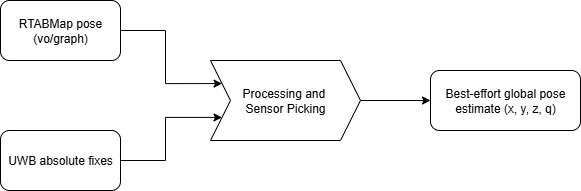
\includegraphics[width=0.85\linewidth]{Images/sensor_fusion.png}
	\caption{Sensor selection and dataflow.}\label{fig-sensor-fusion}
\end{figure}

\subsection*{Sensor fusion contract}
\begin{description}
	\item[Inputs:] RTABMap pose (x, y, z, q), UWB position fixes (x, y, timestamp), IMU measurements (angular velocity, linear acceleration). All inputs are timestamped and published on ROS2 topics.
	\item[Outputs:] A best-effort global pose estimate (x, y, z, q) selected from available sensors; the node republishes the fused pose at a variable rate (typically 10--50\,Hz depending on sensor availability and compute load).
	\item[Error modes:] \begin{itemize}[nosep,leftmargin=*]
		\item \textbf{Missing UWB fixes:} the fusion falls back to visual odometry from RTABMap.
		\item \textbf{Visual tracking loss:} the system holds the last known map pose and uses UWB position with estimated orientation from movement direction; if unsuccessful, it raises an operator-visible warning.
		\item \textbf{Inconsistent UWB readings:} basic validity checks are applied and the system falls back to RTABMap position when UWB appears invalid.
	\end{itemize}
\end{description}

\subsection*{Edge cases and mitigations}
The hybrid localization system must handle several challenging scenarios that can compromise positioning accuracy. Each edge case requires specific detection mechanisms and fallback strategies to maintain system reliability:

\begin{itemize}
	\item \textbf{NLOS UWB measurements:} Non-Line-of-Sight (NLOS) conditions occur when UWB signals reflect off walls or furniture before reaching anchors, causing distance measurements to be longer than the true direct path. This leads to positioning errors that can be several meters off the robot's actual location. The system detects NLOS conditions by comparing UWB-derived positions against RTABMap's visual estimates and checking for sudden position jumps that exceed physically possible robot movement speeds. When NLOS is detected, the fusion logic temporarily ignores UWB fixes and relies solely on RTABMap's visual odometry until consecutive UWB measurements show consistent, physically plausible positions again.
	
	\item \textbf{Feature-poor areas (e.g., blank walls):} Visual SLAM systems like RTABMap require sufficient visual features (corners, textures, patterns) to track camera motion and maintain localization. In environments with blank walls, uniform lighting, or repetitive patterns, the camera may lose tracking or produce unreliable odometry estimates. When RTABMap loses tracking, the system automatically triggers relocalization attempts and informs the VR operator that tracking has been lost and relocalization is in progress. The system relies on the VR user to continue moving the robot (particularly rotating in place) to provide RTABMap with sufficient visual motion to reacquire its position within the existing map. Since UWB typically maintains position estimates, orientation recovery is the primary challenge in these scenarios.
	
	\item \textbf{Camera occlusion by robot fabric:} The Tino robot's fabric covering can occasionally shift during movement and partially obstruct the Oak-D Pro camera's field of view, particularly during rapid rotations or when interacting with humans. This occlusion degrades both RGB image quality for human pose detection and stereo depth estimation reliability. Typically, these occlusion events are brief moments where the fabric temporarily covers the camera before settling back into position, but even these short disruptions can trigger RTABMap relocalization attempts. Currently, the system does not automatically detect or respond to fabric occlusion events - this remains a manual intervention scenario where operators must physically adjust the robot's fabric covering to restore clear camera views when persistent occlusion occurs.
\end{itemize}

\section{Human detection and pose pipeline}

The human perception pipeline is designed to provide real-time 3D skeletons to the VR environment and other behavior nodes. It consists of three stages:

\begin{enumerate}
	\item \textbf{2D detection and pose estimation:} YOLOv11 (TensorRT engine) runs on RGB frames to detect humans and estimate 2D keypoints (17 joints).
	\item \textbf{Depth association:} for each detected joint, the pipeline samples the Oak‑D stereo depth (with median filtering in a small neighbourhood) to recover the joint's metric z coordinate and compute an (x,y,z) in the camera frame.
	\item \textbf{Transform to robot/world frame:} the 3D joint positions are transformed using the current fused global pose to provide world-relative skeletons for VR and navigation.
\end{enumerate}

This multi-stage processing pipeline, from initial RGB input through 2D pose detection to final 3D skeleton output, is illustrated in Figure~\ref{fig-human-pipeline}.

\begin{figure}[H]
	\centering
	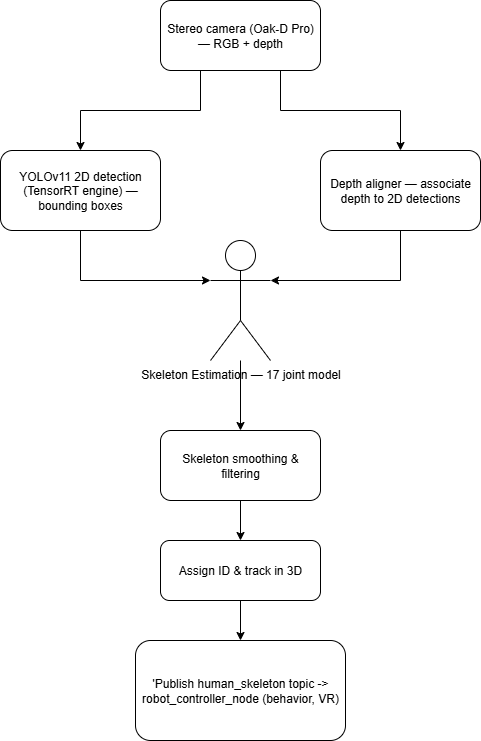
\includegraphics[height=12cm]{Images/human_pipeline.png}
	\caption{Human detection and depth-association pipeline.}\label{fig-human-pipeline}
\end{figure}

The pipeline publishes a \texttt{human\_skeleton} ROS2 message containing a timestamped array of joints, each with position and a confidence score. This message enables downstream nodes to select stable skeletons for interaction logic and VR rendering.

\subsection*{Design contract for perception}
Inputs: synchronized RGB frame, depth image, camera intrinsics, current global pose.
Outputs: timestamped skeletons with 3D joint positions and per-joint confidence.
Failure modes: low confidence joints (reported but flagged), missing depth (use last known depth or drop joint), multiple detections (assign IDs using bounding-box IoU + temporal tracking).

\section{Software architecture and system organisation}

To improve modularity and maintainability the entire robot stack was migrated to ROS2. The project uses a node-based split that mirrors the functional decomposition:

\begin{itemize}
	\item \textbf{Perception:} \texttt{rtabmap} (mapping/localization), \texttt{depthai} camera node, \texttt{yolo11\_pose\_node} (TensorRT inference + skeleton extraction).
	\item \textbf{State and logging:} \texttt{vr\_data\_recorder\_node} (logging for VR and experiments).
	\item \textbf{Control (includes fusion):} \texttt{robot\_controller\_node.py} implements simple sensor selection logic (UWB preferred for position, RTABMap for orientation) and high-level behaviours; \texttt{hardware\_interface\_node.py} handles serial comms to Arduinos using device symlinks \texttt{/dev/ttyHEAD}, \texttt{/dev/ttyBASE}, \texttt{/dev/ttyLEG}.
	\item \textbf{I/O and integration:} \texttt{gamepad\_node.py}, \texttt{audio\_node.py}, \texttt{vr\_interface\_node.py} (VR bridge and topic translation).
\end{itemize}

Design decisions that improved robustness during development included using persistent device symlinks for Arduinos, clearly separated launch files for mapping and localization (\texttt{rtab\_mapping.launch.py}, \texttt{rtab\_localization.launch.py}), and a dedicated VR exporter node that limits published bandwidth and enforces message rate caps for stable VR telepresence.

\section{Implementation notes and rationale from R\&D}

Several practical findings from the development period informed the conceptual choices:

\begin{itemize}
	\item ORB‑SLAM3 and SVO showed compilation and stability problems on ARM64 devices and with older RealSense/T265 hardware; this motivated the switch to RTABMap and the Oak‑D Pro camera.
	\item The Oak‑D Pro + RTABMap standalone build achieved reliable map save/load and relocalization, a key requirement for repeated VR sessions.
	\item Converting YOLOv11 to TensorRT produced the necessary runtime performance for 17-joint skeleton extraction on the Orin Nano while keeping end-to-end latency acceptable for virtual reality.
	\item Power architecture and mechanical changes (new differential base, improved mounts for camera and speakers) reduced vibration and improved perception robustness in the field.
\end{itemize}

\section{Validation plan and quality gates}

To verify the conceptual choices and measure system readiness the following minimal quality gates were defined and executed where possible:

\begin{enumerate}
	\item \textbf{Build and integration:} RTABMap + DepthAI + ROS2 launch files must start and publish \texttt{localization\_pose} and camera topics without crashes for 10 minutes (smoke test).
	\item \textbf{Perception correctness:} YOLOv11 TensorRT skeletons validated against recorded test sequences; per-joint reprojection error to depth must be within 20 cm for frontal poses.
	\item \textbf{Fusion stability:} sensor selection logic must provide reasonable pose estimates when UWB anchors are available, and be able to relocalize to saved maps.
	\item \textbf{End-to-end latency:} perception -> VR message latency measured and kept below 150 ms in typical configurations.
\end{enumerate}

Measured results from the R\&D include:
\begin{itemize}[nosep]
	\item RTABMap with Oak‑D saved and reloaded maps reliably.
	\item YOLOv11 (TensorRT) provided real-time skeletons suitable for VR export.
	\item Orin Nano peak current draw was measured and verified as acceptable after power supply revisions.
\end{itemize}

\section{Summary}

The conceptual framework presented in this chapter establishes the foundation for Tino V2's technical implementation, with each technology choice validated through practical development experience and performance requirements for VR integration.

